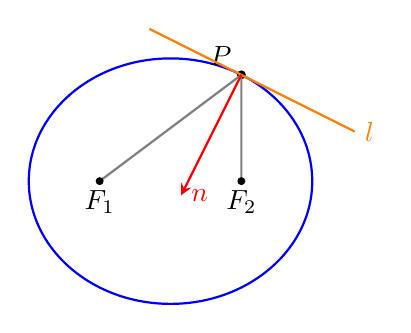
\begin{tikzpicture}[scale=.9,>=stealth]
\draw[blue,thick] (0,0) ellipse (2 and {sqrt(3)});
\coordinate (P) at (1,1.5);\fill (P) circle (1.8pt) node[above left] {$P$};
\draw[gray,thick] (P)--(-1,0);\fill (-1,0) circle (1.6pt) node[below] {$F_1$};
\draw[gray,thick] (P)--(1,0);\fill (1,0) circle (1.6pt) node[below] {$F_2$};
\draw[orange,thick] (-0.30000000000000004,2.15)--(2.6,0.7) node[right] {$l$};
\draw[->,red,thick] (P)--(0.15000000000000002,-0.19999999999999996) node[right] {$n$};
\end{tikzpicture}
